\documentclass[11pt]{article}

\usepackage[a4paper,margin=1in]{geometry}
\usepackage{graphicx}
\usepackage{booktabs}
\usepackage{amsmath}
\usepackage{hyperref}
\usepackage{xcolor}
\usepackage{caption}
\usepackage{listings}
\usepackage{float}
\usepackage{longtable}

\hypersetup{colorlinks=true, linkcolor=blue, urlcolor=blue, citecolor=blue}

\lstset{
  basicstyle=\ttfamily\small,
  breaklines=true,
  frame=single,
  backgroundcolor=\color{gray!10},
  columns=fullflexible
}

\title{\textbf{Experiment 2: Email Spam/Ham Classification using \\ Na\"ive Bayes and KNN}}
\author{Machine Learning Algorithms Laboratory (ICS1512) \\
M.Tech (Integrated) Computer Science and Engineering, Semester V \\
Sri Sivasubramaniya Nadar College of Engineering, Chennai}
\date{}

\begin{document}
\maketitle

\section{Aim and Objective}
To build and compare email spam/ham classifiers using \textbf{Na\"ive Bayes} (Gaussian,
Multinomial, Bernoulli variants) and \textbf{K-Nearest Neighbors (KNN)}, and to:
\begin{itemize}
    \item Compare Gaussian, Multinomial and Bernoulli Na\"ive Bayes.
    \item Study the effect of varying $k$ in KNN.
    \item Compare KDTree and BallTree neighbor search structures.
    \item Optimize KNN using \texttt{GridSearchCV} and \texttt{RandomizedSearchCV}.
    \item Evaluate computational complexity and execution time, both theoretically and experimentally.
    \item Evaluate model stability using $K$-Fold Cross Validation.
\end{itemize}

\section{Theory}

\subsection{Na\"ive Bayes}
Na\"ive Bayes is a probabilistic classifier based on Bayes' theorem, assuming
conditional independence of features given the class:
\begin{equation}
P(C \mid X) = \frac{P(X \mid C)\,P(C)}{P(X)}
\end{equation}
where $C$ is the class label and $X = (x_1, x_2, \ldots, x_d)$ is the feature vector.
Three variants were used, differing in the assumed distribution of $P(x_i \mid C)$:
\begin{itemize}
    \item \textbf{Gaussian NB} assumes each feature is normally distributed within a class.
    \item \textbf{Multinomial NB} models feature counts/frequencies, suited to
    word/character frequency data.
    \item \textbf{Bernoulli NB} models binary presence/absence of a feature.
\end{itemize}

\subsection{K-Nearest Neighbors (KNN)}
KNN is a lazy, instance-based learning algorithm. A query point is classified by
majority vote among its $k$ nearest neighbors in the training set, under a chosen
distance metric (e.g.\ Euclidean, Manhattan). No explicit model is built at training
time; all computation is deferred to prediction time.

\subsection{Neighbor Search Structures: KDTree and BallTree}
Brute-force KNN search is $O(nd)$ per query. \textbf{KDTree} and \textbf{BallTree}
are spatial index structures that partition the training data to accelerate nearest
neighbor queries to $O(\log n)$ on average, at the cost of an $O(n \log n)$ build time.
KDTree partitions space along axis-aligned hyperplanes and tends to work best in
low-to-moderate dimensions, while BallTree partitions data into nested hyperspheres
and is often more robust as dimensionality grows.

\subsection{Hyperparameter Search: GridSearchCV vs.\ RandomizedSearchCV}
\texttt{GridSearchCV} exhaustively evaluates every combination in a specified
parameter grid using cross-validation, guaranteeing the best combination within that
grid at the cost of computation time that grows multiplicatively with the number of
parameters and values. \texttt{RandomizedSearchCV} instead samples a fixed number of
random combinations, trading an exhaustive guarantee for substantially lower
computational cost, and scales better to large search spaces.

\section{Dataset}
The \textbf{Spambase} dataset from the \textbf{UCI Machine Learning Repository}
(dataset id 94, \url{https://archive.ics.uci.edu/dataset/94/spambase}) was used.

\begin{table}[H]
\centering
\caption{Dataset Summary}
\begin{tabular}{ll}
\toprule
\textbf{Item} & \textbf{Value} \\
\midrule
Total samples & 4601 \\
Features & 57 (numeric: word/character frequencies, capital-run-length statistics) \\
Missing values & 0 \\
Duplicate rows & 391 (retained) \\
Class balance & Ham (0): 2788 (60.6\%) \quad Spam (1): 1813 (39.4\%) \\
Train / Test split & 3450 / 1151 (75\% / 25\%, stratified) \\
\bottomrule
\end{tabular}
\end{table}

The dataset was loaded programmatically via the official \texttt{ucimlrepo} package
(with automatic fallback to a direct UCI archive download and a verified mirror of
the same UCI data), so the notebook works end-to-end without depending on Kaggle.

\section{Data Preprocessing}
\begin{enumerate}
    \item \textbf{Missing values:} Spambase has no missing values by construction; the
    pipeline defensively imputes with the column median if any are found.
    \item \textbf{Normalization:} Features were standardized (zero mean, unit variance)
    for Gaussian NB and KNN; Min-Max scaled to $[0,1]$ for Multinomial NB (which
    requires non-negative inputs); and binarized (threshold $=0$) for Bernoulli NB.
\end{enumerate}

\section{Exploratory Data Analysis}

\begin{figure}[H]
\centering
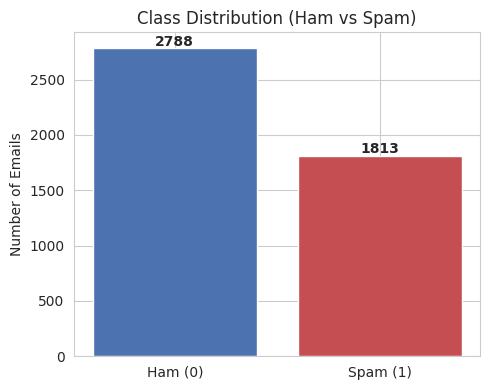
\includegraphics[width=0.55\textwidth]{figs/plot_01_class_distribution.png}
\caption{Class distribution: Ham (2788) vs.\ Spam (1813).}
\end{figure}

\begin{figure}[H]
\centering
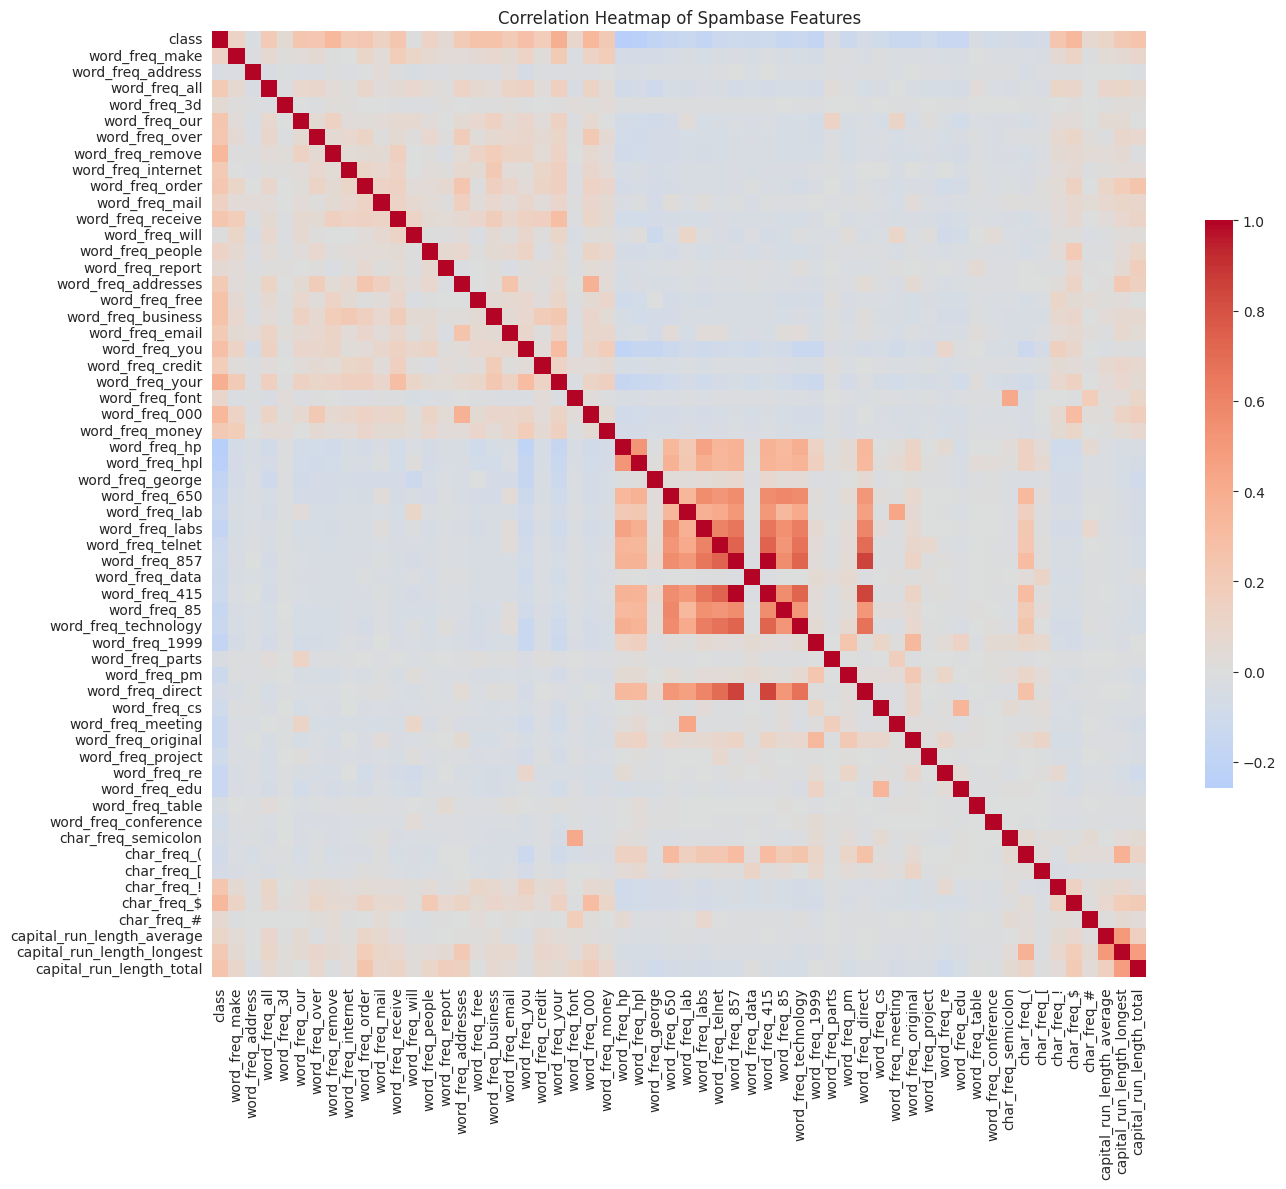
\includegraphics[width=0.85\textwidth]{figs/plot_02_correlation_heatmap.png}
\caption{Correlation heatmap of the 57 Spambase features.}
\end{figure}

The features most correlated with the class label were \texttt{word\_freq\_your},
\texttt{word\_freq\_000}, \texttt{word\_freq\_remove}, \texttt{char\_freq\_\$},
\texttt{word\_freq\_you}, and \texttt{word\_freq\_free}.

\begin{figure}[H]
\centering
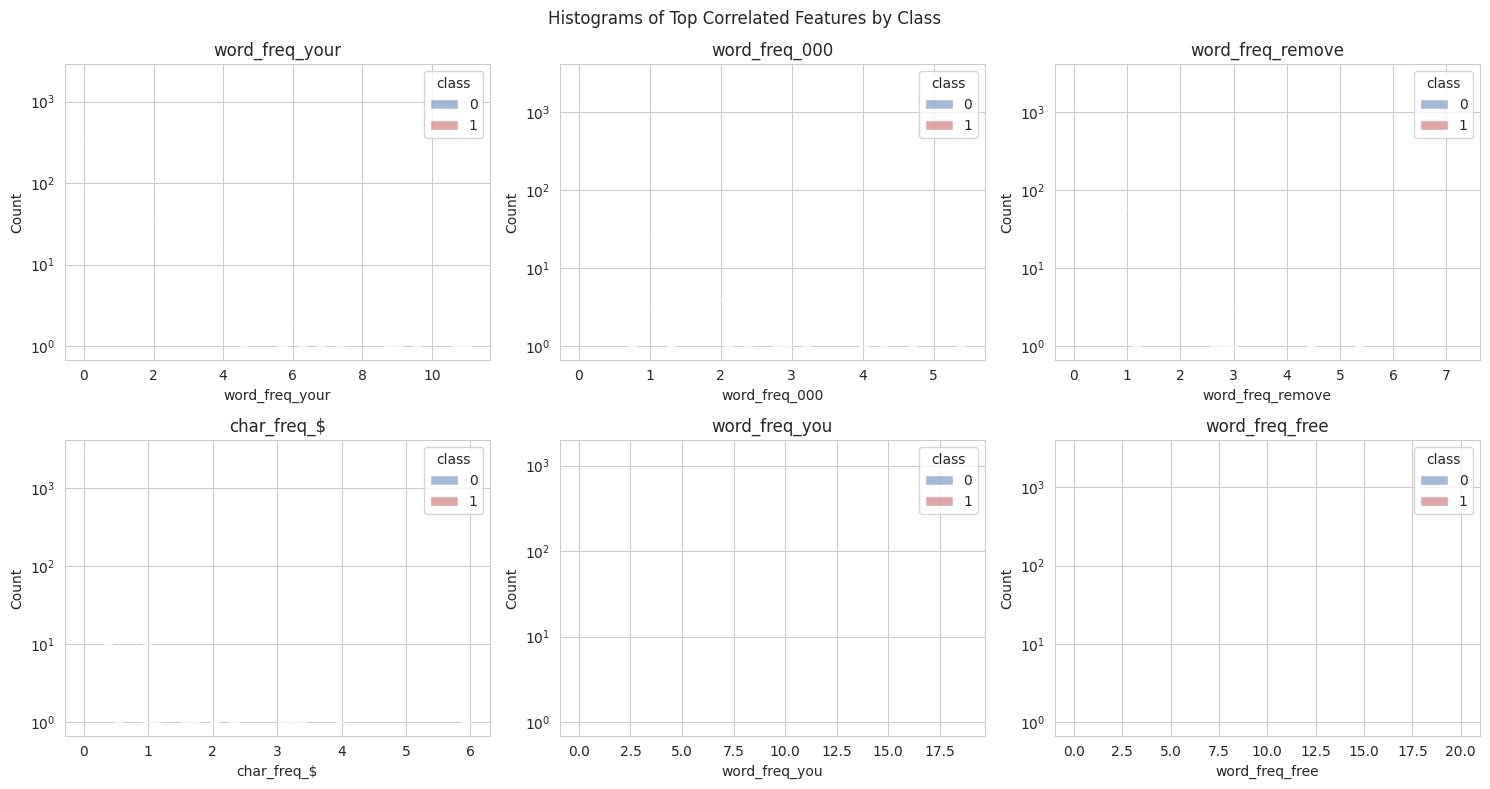
\includegraphics[width=0.95\textwidth]{figs/plot_03_histograms.png}
\caption{Histograms of the top correlated features, split by class.}
\end{figure}

\begin{figure}[H]
\centering
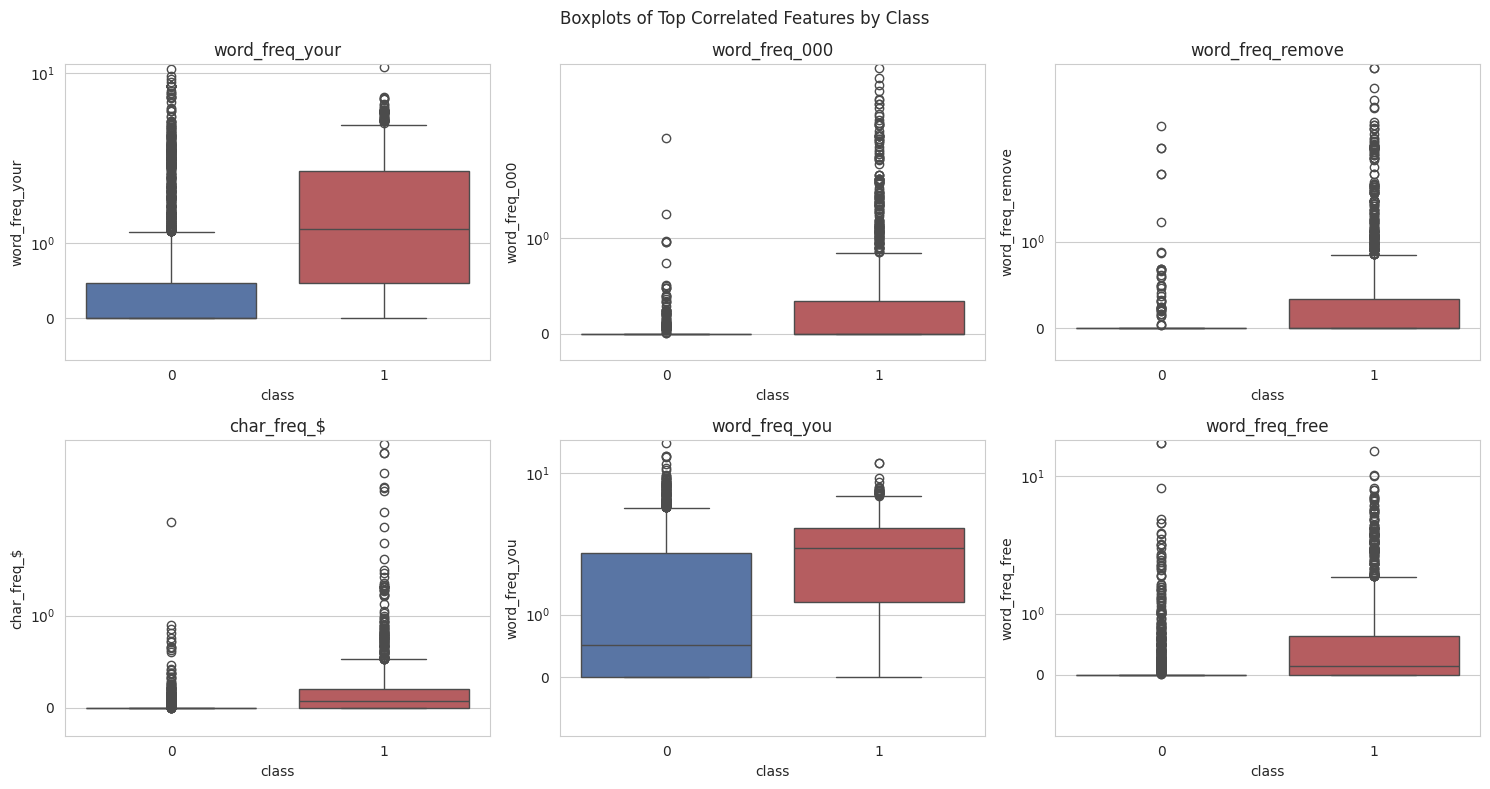
\includegraphics[width=0.95\textwidth]{figs/plot_04_boxplots.png}
\caption{Boxplots of the top correlated features, split by class.}
\end{figure}

\section{Implementation Overview}
The following pipeline was implemented in Python (NumPy, Pandas, Matplotlib, Seaborn,
scikit-learn):
\begin{enumerate}
    \item Load the UCI Spambase dataset.
    \item Handle missing values (none found; defensive median imputation included).
    \item Normalize features (StandardScaler / MinMaxScaler / Binarizer as required per model).
    \item Perform exploratory data analysis.
    \item Stratified train/test split (75/25).
    \item Train Gaussian NB, Multinomial NB, Bernoulli NB, and KNN.
    \item Tune KNN using \texttt{GridSearchCV}.
    \item Tune KNN using \texttt{RandomizedSearchCV}.
    \item Compare KDTree and BallTree search algorithms.
    \item Perform 5-fold stratified cross-validation.
    \item Measure training and prediction time for every model.
    \item Generate all required evaluation plots.
\end{enumerate}

A representative code snippet for model evaluation:
\begin{lstlisting}[language=Python]
def evaluate_model(name, model, X_tr, y_tr, X_te, y_te):
    t0 = time.perf_counter()
    model.fit(X_tr, y_tr)
    train_time = time.perf_counter() - t0

    t0 = time.perf_counter()
    y_pred = model.predict(X_te)
    predict_time = time.perf_counter() - t0

    y_proba = model.predict_proba(X_te)[:, 1]
    return {
        'Accuracy': accuracy_score(y_te, y_pred),
        'Precision': precision_score(y_te, y_pred),
        'Recall': recall_score(y_te, y_pred),
        'F1': f1_score(y_te, y_pred),
        'ROC-AUC': roc_auc_score(y_te, y_proba),
        'Train Time (s)': train_time,
        'Predict Time (s)': predict_time,
    }
\end{lstlisting}
The full, executed implementation is provided in the accompanying Jupyter notebook
\texttt{Experiment\_2\_Spam\_Classification.ipynb}.

\section{Results}

\subsection{Na\"ive Bayes Comparison}
\begin{table}[H]
\centering
\caption{Na\"ive Bayes Comparison}
\begin{tabular}{lccc}
\toprule
\textbf{Metric} & \textbf{Gaussian} & \textbf{Multinomial} & \textbf{Bernoulli} \\
\midrule
Accuracy  & 0.8254 & \textbf{0.9001} & 0.8818 \\
Precision & 0.7077 & \textbf{0.9472} & 0.8768 \\
Recall    & \textbf{0.9493} & 0.7907 & 0.8150 \\
F1        & 0.8109 & \textbf{0.8619} & 0.8447 \\
ROC-AUC   & 0.9368 & \textbf{0.9614} & 0.9503 \\
\bottomrule
\end{tabular}
\end{table}

Multinomial NB achieved the best accuracy, precision, F1 and ROC-AUC, matching the
count-based nature of the frequency features. Gaussian NB obtained the highest recall
but lowest precision, since its normal-distribution assumption is a poor fit for these
sparse, skewed features.

\begin{figure}[H]
\centering
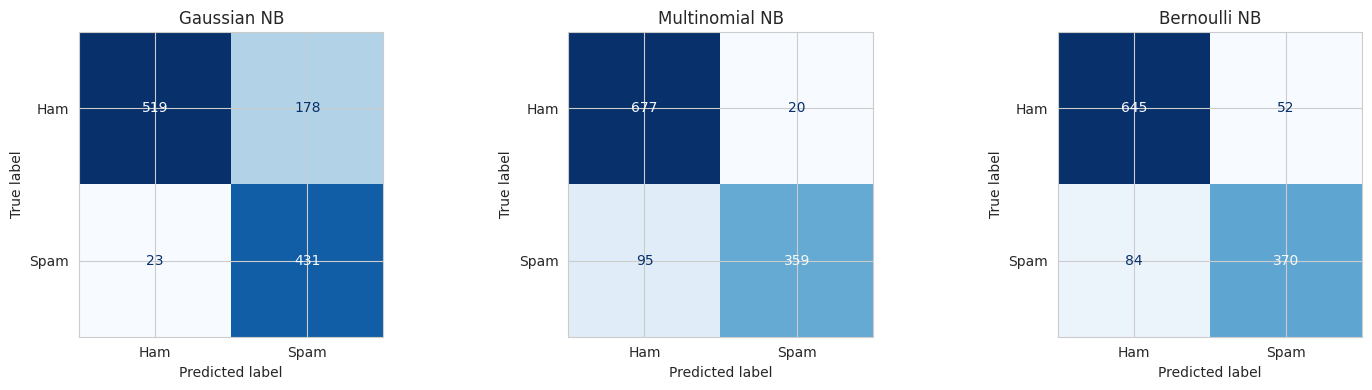
\includegraphics[width=0.95\textwidth]{figs/plot_05a_confusion_matrices_nb.png}
\caption{Confusion matrices for Gaussian, Multinomial, and Bernoulli NB.}
\end{figure}

\subsection{KNN — Effect of Varying $k$}
\begin{table}[H]
\centering
\caption{KNN Comparison (Euclidean distance, uniform weights)}
\begin{tabular}{lcccc}
\toprule
\textbf{k} & \textbf{Accuracy} & \textbf{Precision} & \textbf{Recall} & \textbf{F1} \\
\midrule
1  & 0.8975 & 0.8733 & 0.8656 & 0.8695 \\
3  & 0.9018 & 0.8814 & 0.8678 & 0.8746 \\
5  & 0.8992 & 0.8789 & 0.8634 & 0.8711 \\
7  & 0.9053 & 0.8929 & 0.8634 & 0.8779 \\
9  & \textbf{0.9062} & 0.8932 & 0.8656 & 0.8792 \\
11 & 0.9027 & 0.8904 & 0.8590 & 0.8744 \\
\bottomrule
\end{tabular}
\end{table}

\begin{figure}[H]
\centering
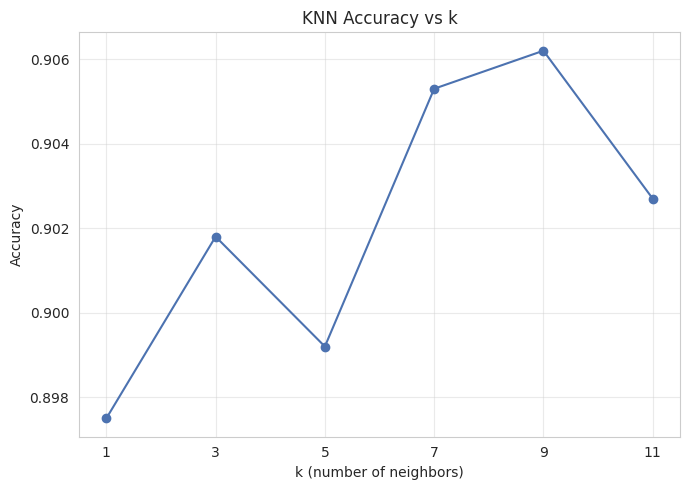
\includegraphics[width=0.6\textwidth]{figs/plot_08_accuracy_vs_k.png}
\caption{KNN accuracy vs.\ $k$. Best plain KNN: $k=9$, accuracy $=0.9062$.}
\end{figure}

\subsection{Hyperparameter Tuning: GridSearchCV vs.\ RandomizedSearchCV}
\begin{table}[H]
\centering
\caption{GridSearchCV vs.\ RandomizedSearchCV (KNN)}
\begin{tabular}{lcc}
\toprule
\textbf{Parameter} & \textbf{GridSearchCV} & \textbf{RandomizedSearchCV} \\
\midrule
Best $k$          & 13        & 6 \\
Metric             & manhattan & manhattan \\
Weights            & distance  & distance \\
Algorithm          & ball\_tree & kd\_tree \\
CV Accuracy        & 0.9241    & \textbf{0.9249} \\
Execution Time (s) & 41.19     & \textbf{16.82} \\
\bottomrule
\end{tabular}
\end{table}

\begin{figure}[H]
\centering
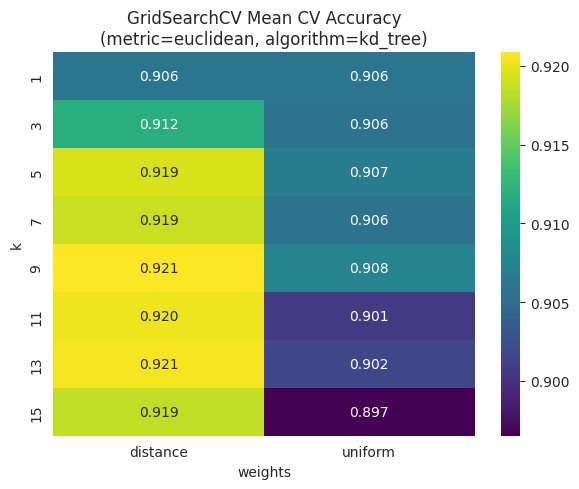
\includegraphics[width=0.55\textwidth]{figs/plot_13_gridsearch_heatmap.png}
\caption{GridSearchCV mean CV accuracy heatmap (metric=euclidean, algorithm=kd\_tree).}
\end{figure}

\begin{figure}[H]
\centering
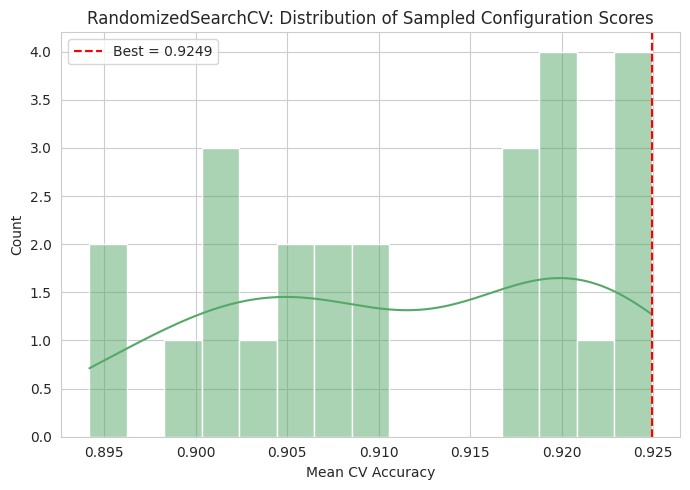
\includegraphics[width=0.6\textwidth]{figs/plot_14_randomsearch_distribution.png}
\caption{Distribution of mean CV accuracy across RandomizedSearchCV's sampled configurations.}
\end{figure}

Both searches converge on \emph{Manhattan distance} with \emph{distance-weighted}
voting as the strongest configuration. RandomizedSearchCV reached a marginally higher
CV accuracy in about $41\%$ of GridSearchCV's execution time by sampling only 25 of
the 64 possible grid combinations.

\subsection{Best Tuned KNN}
Best parameters (GridSearchCV): \texttt{algorithm=ball\_tree, metric=manhattan,
n\_neighbors=13, weights=distance}.

\begin{table}[H]
\centering
\caption{Best Tuned KNN — Full Evaluation}
\begin{tabular}{lc}
\toprule
\textbf{Metric} & \textbf{Value} \\
\midrule
Accuracy          & 0.9209 \\
Precision         & 0.9504 \\
Recall            & 0.8436 \\
F1                & 0.8938 \\
ROC-AUC           & 0.9754 \\
Train Time (s)    & 0.0213 \\
Predict Time (s)  & 0.2531 \\
\bottomrule
\end{tabular}
\end{table}

\begin{figure}[H]
\centering
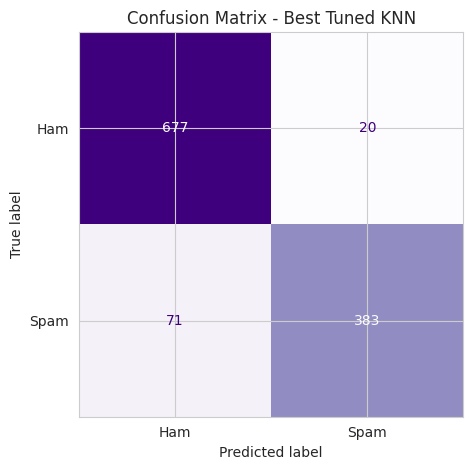
\includegraphics[width=0.4\textwidth]{figs/plot_05b_confusion_matrix_best_knn.png}
\caption{Confusion matrix — Best tuned KNN.}
\end{figure}

\subsection{KDTree vs.\ BallTree}
\begin{table}[H]
\centering
\caption{KDTree vs.\ BallTree}
\begin{tabular}{lccc}
\toprule
\textbf{Metric} & \textbf{KDTree} & \textbf{BallTree} \\
\midrule
Accuracy             & 0.9209 & 0.9209 \\
Training Time (s)    & 0.0167 & \textbf{0.0091} \\
Prediction Time (s)  & 0.2864 & \textbf{0.2404} \\
\bottomrule
\end{tabular}
\end{table}

Both structures give identical accuracy (they compute exact nearest neighbors);
BallTree was faster for both training and prediction on this 57-dimensional dataset.

\subsection{5-Fold Cross Validation}
\begin{table}[H]
\centering
\caption{5-Fold Cross Validation: Best Na\"ive Bayes vs.\ Best KNN}
\begin{tabular}{lcc}
\toprule
\textbf{Fold} & \textbf{Na\"ive Bayes (Multinomial)} & \textbf{Best KNN} \\
\midrule
1 & 0.8855 & 0.9130 \\
2 & 0.8971 & 0.9232 \\
3 & 0.8942 & 0.9420 \\
4 & 0.8826 & 0.9261 \\
5 & 0.8812 & 0.9159 \\
\midrule
\textbf{Average} & \textbf{0.8881} & \textbf{0.9240} \\
\bottomrule
\end{tabular}
\end{table}

\begin{figure}[H]
\centering
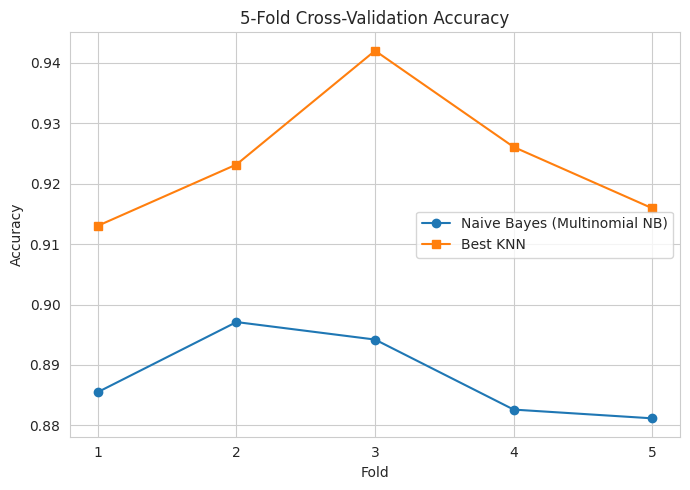
\includegraphics[width=0.6\textwidth]{figs/plot_09_cv_accuracy.png}
\caption{5-Fold cross-validation accuracy per fold.}
\end{figure}

The tuned KNN model consistently outperforms Multinomial NB across every fold,
confirming the stability of its higher test accuracy.

\section{Complexity Analysis}

\subsection{Theoretical Time Complexity}
\begin{table}[H]
\centering
\caption{Theoretical Time Complexity ($n$ = training samples, $d$ = features)}
\begin{tabular}{lcc}
\toprule
\textbf{Algorithm} & \textbf{Training} & \textbf{Prediction} \\
\midrule
Na\"ive Bayes    & $O(nd)$      & $O(d)$ \\
KNN (Brute)      & $O(1)$       & $O(nd)$ \\
KDTree           & $O(n\log n)$ & $O(\log n)_{\text{avg}}$ \\
BallTree         & $O(n\log n)$ & $O(\log n)_{\text{avg}}$ \\
\bottomrule
\end{tabular}
\end{table}

\subsection{Experimental Time Analysis}
\begin{table}[H]
\centering
\caption{Experimental Time Analysis ($n\approx3450$ train, $\approx1151$ test, $d=57$)}
\begin{tabular}{lcc}
\toprule
\textbf{Algorithm} & \textbf{Training (s)} & \textbf{Prediction (s)} \\
\midrule
Gaussian NB     & 0.0144 & 0.0007 \\
Multinomial NB  & \textbf{0.0021} & \textbf{0.0002} \\
Bernoulli NB    & 0.0036 & 0.0011 \\
Best KNN        & 0.0092 & \textbf{0.2358} \\
\bottomrule
\end{tabular}
\end{table}

\begin{figure}[H]
\centering
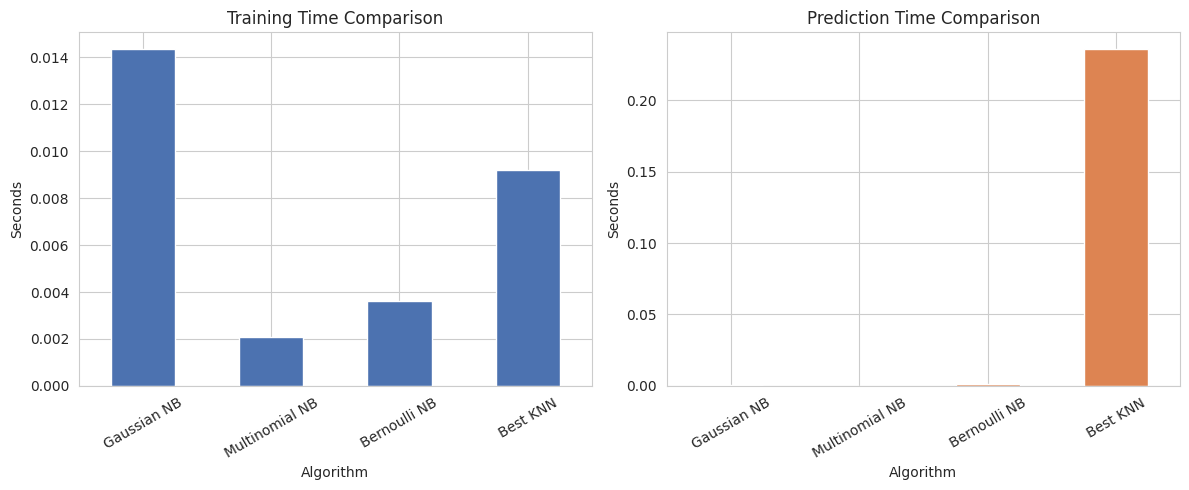
\includegraphics[width=0.95\textwidth]{figs/plot_10_11_time_comparison.png}
\caption{Training time and prediction time comparison across all models.}
\end{figure}

The measured times closely track theory: all Na\"ive Bayes variants train and predict
in a few milliseconds, while KNN's prediction time is two to three orders of magnitude
larger, since it must search neighbors at query time for every test point even with a
tree-based index. KNN's training time is negligible, as it is a lazy learner that
merely stores the training data (and, when applicable, builds the tree index).

\section{Additional Evaluation Plots}

\begin{figure}[H]
\centering
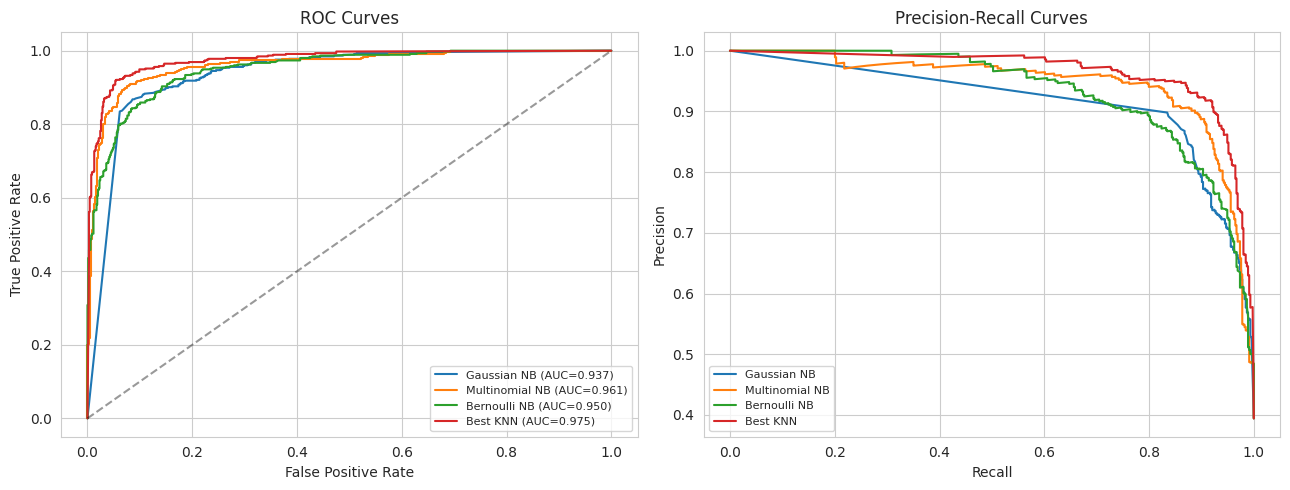
\includegraphics[width=0.95\textwidth]{figs/plot_06_07_roc_pr_curves.png}
\caption{ROC curves and Precision-Recall curves for all models.}
\end{figure}

\begin{figure}[H]
\centering
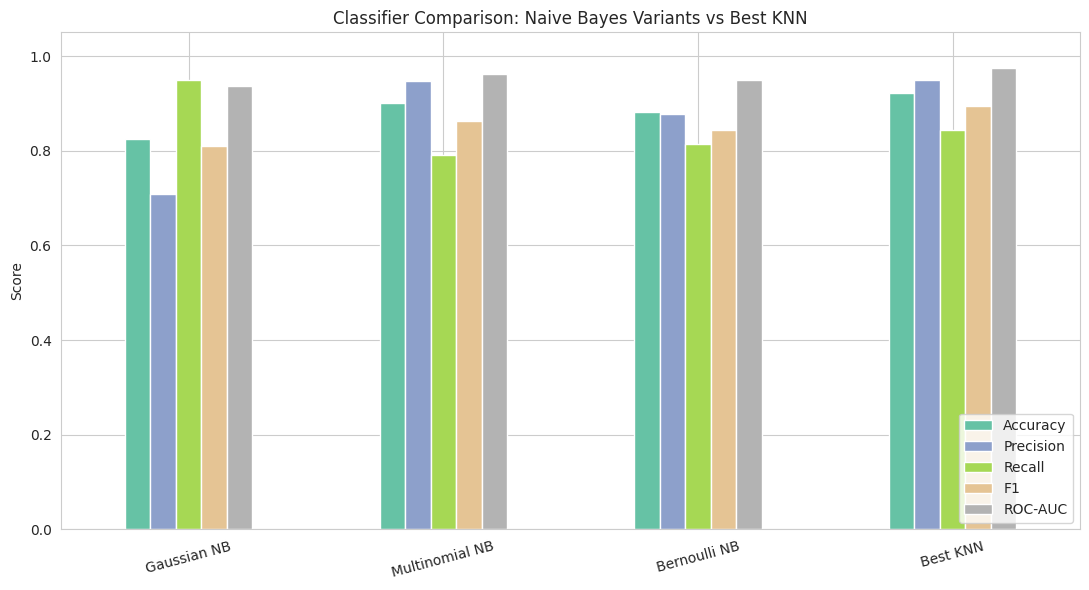
\includegraphics[width=0.85\textwidth]{figs/plot_12_classifier_comparison.png}
\caption{Overall classifier comparison across Accuracy, Precision, Recall, F1 and ROC-AUC.}
\end{figure}

\begin{table}[H]
\centering
\caption{Overall Classifier Comparison}
\begin{tabular}{lccccc}
\toprule
\textbf{Model} & \textbf{Accuracy} & \textbf{Precision} & \textbf{Recall} & \textbf{F1} & \textbf{ROC-AUC} \\
\midrule
Gaussian NB           & 0.8254 & 0.7077 & \textbf{0.9493} & 0.8109 & 0.9368 \\
Multinomial NB        & 0.9001 & \textbf{0.9472} & 0.7907 & 0.8619 & 0.9614 \\
Bernoulli NB          & 0.8818 & 0.8768 & 0.8150 & 0.8447 & 0.9503 \\
\textbf{Best KNN (tuned)} & \textbf{0.9209} & 0.9504 & 0.8436 & \textbf{0.8938} & \textbf{0.9754} \\
\bottomrule
\end{tabular}
\end{table}

\section{Additional Tasks}

\subsection{Effect of Train-Test Split Ratio (Tuned KNN)}
\begin{table}[H]
\centering
\begin{tabular}{lcc}
\toprule
\textbf{Test Size} & \textbf{Train Size} & \textbf{Accuracy} \\
\midrule
0.1 & 0.9 & 0.9046 \\
0.2 & 0.8 & 0.9164 \\
0.3 & 0.7 & \textbf{0.9247} \\
0.4 & 0.6 & 0.9158 \\
\bottomrule
\end{tabular}
\end{table}
Accuracy remains stable (0.90--0.92) across split ratios, peaking near a 70/30 split.

\subsection{Euclidean vs.\ Manhattan Distance}
\begin{table}[H]
\centering
\begin{tabular}{lcc}
\toprule
\textbf{Distance} & \textbf{Accuracy} & \textbf{F1} \\
\midrule
Euclidean  & 0.9140 & 0.8894 \\
\textbf{Manhattan} & \textbf{0.9209} & \textbf{0.8938} \\
\bottomrule
\end{tabular}
\end{table}
Manhattan distance outperforms Euclidean, consistent with the tuning result, likely
because it is less sensitive to the outliers/skew present in the frequency features.

\subsection{Weighted vs.\ Uniform KNN}
\begin{table}[H]
\centering
\begin{tabular}{lcc}
\toprule
\textbf{Weighting} & \textbf{Accuracy} & \textbf{F1} \\
\midrule
Uniform   & 0.9027 & 0.8670 \\
\textbf{Distance}  & \textbf{0.9209} & \textbf{0.8938} \\
\bottomrule
\end{tabular}
\end{table}
Distance-weighted voting clearly improves both accuracy and F1 over uniform voting.

\subsection{Overfitting vs.\ Underfitting in KNN}
A very small $k$ (e.g.\ $k=1$) makes KNN sensitive to noise and outliers in the
training data, causing the decision boundary to become highly irregular and the model
to \textbf{overfit}. A very large $k$ oversmooths the boundary by averaging over many,
possibly irrelevant, distant neighbors, causing the model to \textbf{underfit} and lose
sensitivity to local structure. The accuracy-vs-$k$ curve (Figure~5) reflects this: it
rises then plateaus/dips, and the best generalizing configuration found by
\texttt{GridSearchCV} used a moderate $k=13$ combined with distance weighting.

\section{Analysis Questions}
\begin{enumerate}
    \item \textbf{Which Na\"ive Bayes variant performed best?} Multinomial NB
    (Accuracy 0.9001, F1 0.8619, ROC-AUC 0.9614) — its count-based event model best
    matches word/character frequency features.
    \item \textbf{What is the optimal value of $k$?} $k=13$ with distance weighting and
    Manhattan distance (GridSearchCV); the best plain (unweighted, Euclidean) $k$ was 9.
    \item \textbf{Compare GridSearchCV and RandomizedSearchCV.} RandomizedSearchCV
    reached a slightly higher CV accuracy (0.9249 vs.\ 0.9241) in 16.82s vs.\ 41.19s
    ($\sim$2.4$\times$ faster) by sampling only 25 of 64 possible combinations.
    \item \textbf{Compare KDTree and BallTree.} Identical accuracy (both exact); BallTree
    was faster here for both training and prediction.
    \item \textbf{Compare theoretical and practical complexity.} Practical timings
    matched theory: Na\"ive Bayes trains/predicts in milliseconds; KNN prediction is by
    far the most expensive step, consistent with its $O(nd)$ / $O(\log n)_\text{avg}$
    complexity versus Na\"ive Bayes' $O(d)$ prediction cost.
    \item \textbf{Which classifier is preferred for large datasets?} Na\"ive Bayes —
    its linear-in-$n$ training and near-constant prediction cost per query scale far
    better than KNN, whose prediction cost grows with the size of the reference dataset
    even with a tree index.
\end{enumerate}

\section{Conclusion}
Across all metrics, the \textbf{tuned KNN model} ($k=13$, Manhattan distance,
distance-weighted, BallTree algorithm) was the strongest overall classifier
(Accuracy 0.9209, F1 0.8938, ROC-AUC 0.9754), narrowly ahead of \textbf{Multinomial
NB} (Accuracy 0.9001, ROC-AUC 0.9614). However, KNN's prediction time
($\sim$0.24\,s for 1151 test points) is roughly 100--1000$\times$ slower than any
Na\"ive Bayes variant, so for very large-scale or latency-sensitive spam filtering,
\textbf{Multinomial Na\"ive Bayes} remains the more practical choice, while tuned KNN
is preferable when maximum accuracy is the priority and the dataset size is moderate.

\section*{References}
\begin{itemize}
    \item Scikit-learn Documentation, \url{https://scikit-learn.org}
    \item Aur\'elien G\'eron, \emph{Hands-On Machine Learning with Scikit-Learn, Keras
    and TensorFlow}
    \item Christopher M.\ Bishop, \emph{Pattern Recognition and Machine Learning}
    \item Dua, D.\ and Graff, C.\ (2019). UCI Machine Learning Repository, Spambase
    Data Set. Irvine, CA: University of California, School of Information and Computer
    Science. \url{https://archive.ics.uci.edu/dataset/94/spambase}
\end{itemize}

\end{document}
